\documentclass[11pt]{beamer}
\usepackage[MeX]{polski}
\usepackage[utf8]{inputenc}
\usepackage{amsmath}
\usepackage{amsfonts}
\usepackage{amssymb}
\usepackage{graphicx}
\usetheme{CambridgeUS}
\usecolortheme{beaver}
\usepackage{textpos}
\begin{document}
	\author[M.R, S.Z, B.D, M.Z, J.H.]{Monika Richter, Sebastian Zając, Bartosz Dziewit \\ Marek Zralek, Jacek Holeczek}
	\title[Symetria zapachowa w MS i poza MS]{Dyskretne grupy symetrii zapachowej w Modelu Standardowym i w modelach Nowej Fizyki}
	%\logo{}
	\institute[WMP, IF]{WMP.SNŚ UKSW\\ IF UŚ}
	\date{\today}
	%\subject{}
	%\setbeamercovered{transparent}
	%\setbeamertemplate{navigation symbols}{}
	\begin{frame}	
			\maketitle
	\end{frame}
		
\section{Model Standardowy cząstek elementarnych}
\begin{frame}
\frametitle{Model Standardowy (MS)}
MS opisuje znane cząstki elementarne i ich oddziaływania, ale jest teorią efektywną.
\begin{center}
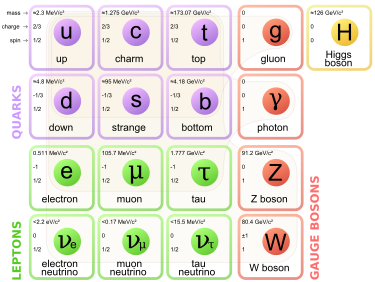
\includegraphics[scale=0.5]{SM.png}
\end{center}
\end{frame}
\begin{frame}
\frametitle{Problemy MS}
\begin{block}{Model Standardowy}
\begin{itemize}
\item Duża liczba wolnych parametrów (25 lub 27),
\item Trzy rodziny cząstek,
\item Hierarchia mas fermionów
\item ...
\end{itemize}
\end{block}
\begin{block}{Neutrina}
\begin{itemize}
\item Czy neutrina to cząstki Diraca czy Majorany ? 
\item Jaki jest mechanizm nabywania masy dla neutrin ? 
\item Jaka jest masa najlżejszego neutrina ?
\item Normalna bądź odwrócona hierarchia mas neutrin ?
\item Dlaczego masa neutrin jest tak mała w porównaniu do innych leptonów ?
\end{itemize}
\end{block}
\end{frame}
\section{Masa leptonów}
\begin{frame}
\frametitle{Masy leptonów}
\begin{block}{Człony Yukawy}
Za generowanie mas fermionów odpowiedzialna jest część Yukawy Lagranżjanu MS. W przypadku neutrin Diraca :
$$\mathcal{L}_Y=-\sum_{\alpha,\beta=e,\mu,\tau}\left[ Y^{'l}_{\alpha\beta}\bar{L}'_{\alpha L} \Phi l'_{\beta R} + Y^{'\nu}_{\alpha\beta} \bar{L}'_{\alpha L} \tilde{\Phi}\nu'_{\beta R}\right] + h.c$$
gdzie: $Y^{'l},Y^{'\nu}$ to macierze Yukawy, $L'_{\alpha L}= {v_{\alpha L} \choose l_{\alpha L}}$ dublet lewoskrętnych leptonów, $l'_R,\nu'_R$ to singlety prawoskrętnych leptonów. Pole Higgsa $\tilde{\Phi}=i\sigma_2\Phi^{\ast}$
\end{block}
Po złamaniu symetrii.  $\Phi = \frac{1}{\sqrt{2}}{0 \choose v+H}$ oraz po diagonalizacji macierzy Yukawy $$V_L^l Y^l V_R^l = Y^l = diag(m_e,m_{\mu},m_{\tau}) $$
$$V_L^{\nu}Y^{'\nu}V_R^\nu = Y^{\nu} = diag(m_1,m_{2},m_{3}) $$
\end{frame}
\section{Macierz Mieszania}
\frame{
\frametitle{Masy leptonów}
\begin{block}{Otrzymujemy człony masowe}
$$\mathcal{L}_Y=-\sum_{\alpha = e,\mu,\tau }\frac{y^l_{\alpha}}{\sqrt{2}}\bar{l}_{\alpha}l_{\alpha} -\sum_{k = 1,2,3 }\frac{y^{\nu}_{k}}{\sqrt{2}}\bar{\nu}_{k}\nu_{k} $$
gdzie masy leptonów:
$$m_{k}=\frac{y^{\nu}_{k} v}{\sqrt{2}},\quad m_\alpha=\frac{y^{l}_{\alpha} v}{\sqrt{2}}$$
\end{block}
\begin{block}{Definicja leptonowej macierzy mieszania}
$$j^{\mu}_{W,L} = 2\bar{\nu}'_L\gamma^{\mu}l'_L =2\bar{\nu}_L V^{\nu \dagger}_LV^{l}_L\gamma^{\mu}l_L  = 2\bar{\nu}_L U^{\dagger}_{PMNS}\gamma^{\mu}l_L$$
Macierz $U_{PMNS}$ parametryzowana jest przez 3 kąty i jedną fazę (CP phase)
\end{block}
}

\frame{
\frametitle{Macierz mieszania}
\begin{center}
	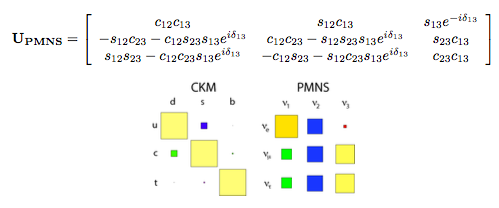
\includegraphics[scale=0.65]{rys4.png}
\end{center}
}
\section{Symetria zapachowa przed i po 2012}
\begin{frame}{Symetria zapachowa przed i po 2012}
\begin{block}{CEL:}
	{\bf Wyjaśnić parametry macierzy mieszania !!! poprzez rozszerzenie grupy symetrii gauge o dyskretną grupę symetrii zapachowej}
\end{block}
Przed 2012 rokiem kąt $\theta_{13}= 0$. 

Grupą symetrii realizującą wartości eksperymentalne była grupa $A_4$ ($S_4,\Delta(27),\Delta(54),...$). Generowała ona następującą macierz mieszania: 
 \begin{center}
 	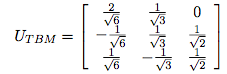
\includegraphics[scale=0.8]{rys5.png}
 \end{center}
\end{frame}
\frame{
\frametitle{Symetria zapachowa przed i po 2012}
Po 2012 postać $U_{TBM}$ trzeba było odrzucić -- $\theta_{13}\neq 0$ 

Nowe modele wyjaśniające parametry macierzy mieszania bazujące na złamaniu symetrii zapachowej: $\Delta(96)$, $\Delta(384)$, $\Delta(600)$ (zachowanie CP). A co z masami ? 
\begin{block}{Podsumowanie modeli w MS}
	\begin{center}
{\bf Żaden model nie przewiduje mas leptonów naładowanych oraz neutrin }
	\end{center}
\end{block}
\begin{block}{Lemat Schura}
Jeśli $T$ jest nieredukowalną reprezentacją skończonej grupy $G$ oraz $$T(g)^{\dagger}MT(g) = M , \quad \forall g\in G$$ 
wtedy macierz $M = \lambda I$.
\end{block}
A może trzeba wyjść poza Model Standardowy ?
}

\section{Modele Nowej Fizyki - Two Higgs Doublet Model}
\begin{frame}{Two Higgs Doublet Model (THDM type III)}
\begin{block}{Motywacja}
Jedno z podstawowych rozszerzeń MS to model z dwoma dubletami Higgsa. Dla ułatwienia rozważmy jedną część Lagranżjanu Yukawy:
$$\mathcal{L}_Y=-\bar{L}'_{L}(Y^{'l}_{j} \Phi_{j}) l'_{R} $$
Wybierzmy pewną nie-abelową, dyskretną grupę $\mathbb{G}_F$
$$L'_L\to A_L L'_L,\quad l'_R \to A_l l'_R, \quad\Phi \to A_{\phi} \Phi,$$
gdzie $A_L, A_l$ 3-wymiarowe nieredukowalne reprezentacje grupy zapachowej, 
natomiast $A_\phi$ 2-wymiarowa nieredukowalna reprezentacja grupy zapachowej.
\end{block}

\end{frame}
\frame{\frametitle{Zadanie do rozwiązania:}
$$A_L(f)^{\dagger}(Y_j(A_\phi)_{jk}(f))A_R(f)=Y_k, \quad \forall f\in G$$
\begin{itemize}
\item Znajdź rozwiązanie równania własnego: $N(f)Y'^{l}=Y'^{l}$ otrzymujemy postać macierzy Yukawy. 
\item Z macierzy Yukawy stwórz macierz masową $M'^{\nu, l}=\frac{1}{\sqrt{2}}v_iY'^{\nu, l}_i$
\item Zdiagonalizuj macierze $M'^{l}, M'^{\nu}$
\item Iloczyn macierzy diagonalizujących = $U_{MNPS}$
\end{itemize}
}
\section{Podsumowanie}
\frame{
\frametitle{Podsumowanie}
\begin{itemize}
\item Analizie poddane zostały, dyskretne, nie-abelowe podgrupy  $U(3)$ do rzędu $1025$ (biblioteka GAP).
\item Zarówno w przypadku MS jak i modeli z rozszerzonym sektorem Higgsa macierz mieszania sprowadza się do macierzy diagonalnej.
\item Rozszerzenie sektora Higgsa {\bf NIE} jest wystarczające aby z symetrii dyskretnej wyznaczyć masy leptonów naładowanych i neutrin.
\item A może bardziej ogólne oddziaływania ? 
\end{itemize}
}
\end{document}